\chapter{物理样机实验验证}\label{chap:experiment}

本章在物理样机上对第四章的控制方案进行验证，按原地平衡、速度跟踪、腿长控制和滚转稳定四个工况依次展开。记录的数据包括机体俯仰角 $\theta_b$、滚转角 $\gamma$、前进速度 $\dot{s}$、左右虚拟腿长 $l_l,l_r$、轮端力矩 $T_{lw,l},T_{lw,r}$ 和腿部关节力矩 $\tau_l,\tau_r$。俯仰角和速度用来评估 LQR 的平衡与跟踪表现，腿长及关节力矩用来检查 VMC 腿长通道的实际支撑效果，滚转角和腿长差用来判断侧向补偿是否起作用。
\section{物理样机平台介绍}

实验样机由机械本体、驱动系统、传感系统、嵌入式控制系统和上位机记录系统组成。机械部分沿用第二章提出的混合式双轮足结构，左右腿均采用对称闭环连杆机构，足端安装轮毂电机。腿部关节电机布置在靠近躯干的位置，并通过链传动驱动连杆运动，从而在保证腿部运动范围的同时减小末端转动惯量。

\begin{figure}[H]
  \centering
  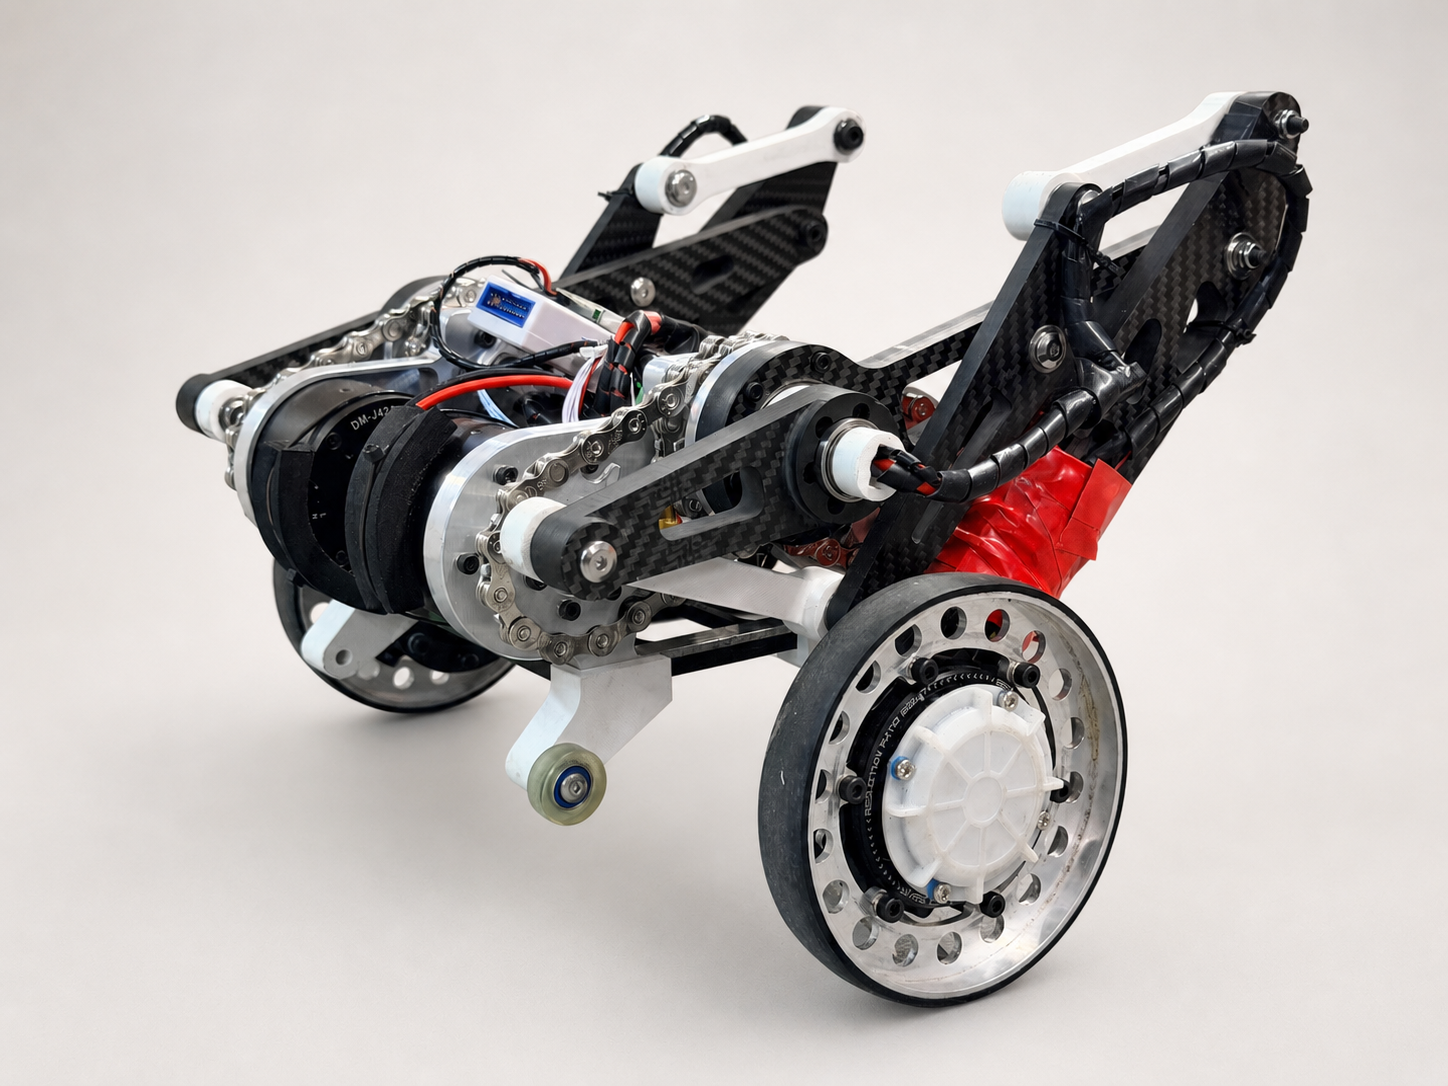
\includegraphics[width=0.85\textwidth]{figures/ch05/demo.png}
  \caption{物理样机实物图}
\end{figure}

控制程序部署在 STM32H723 主控板上，主频为 $480\,\mathrm{MHz}$。每个控制周期内，主控板读取惯性测量单元、轮毂电机编码器和腿部关节编码器的数据，并按照第四章的状态估计方法更新机体姿态、前进速度、虚拟腿长和腿摆角。随后，程序计算 LQR 输出的轮端力矩与腿摆控制量、VMC 输出的腿长支撑力以及滚转修正量，再将对应力矩指令发送给各电机驱动器。

传感器布置与状态估计量一一对应。惯性测量单元安装在机体中部附近，直接给出俯仰角、滚转角及角速度；轮毂电机编码器提供左右轮角速度，并参与前进速度估计；腿部关节编码器结合第三章的五连杆运动学关系，解算左右虚拟腿长和腿摆角。实验数据由上位机通过无线烧录器记录，实验结束后再离线绘图和分析。

\begin{figure}[H]
  \centering
  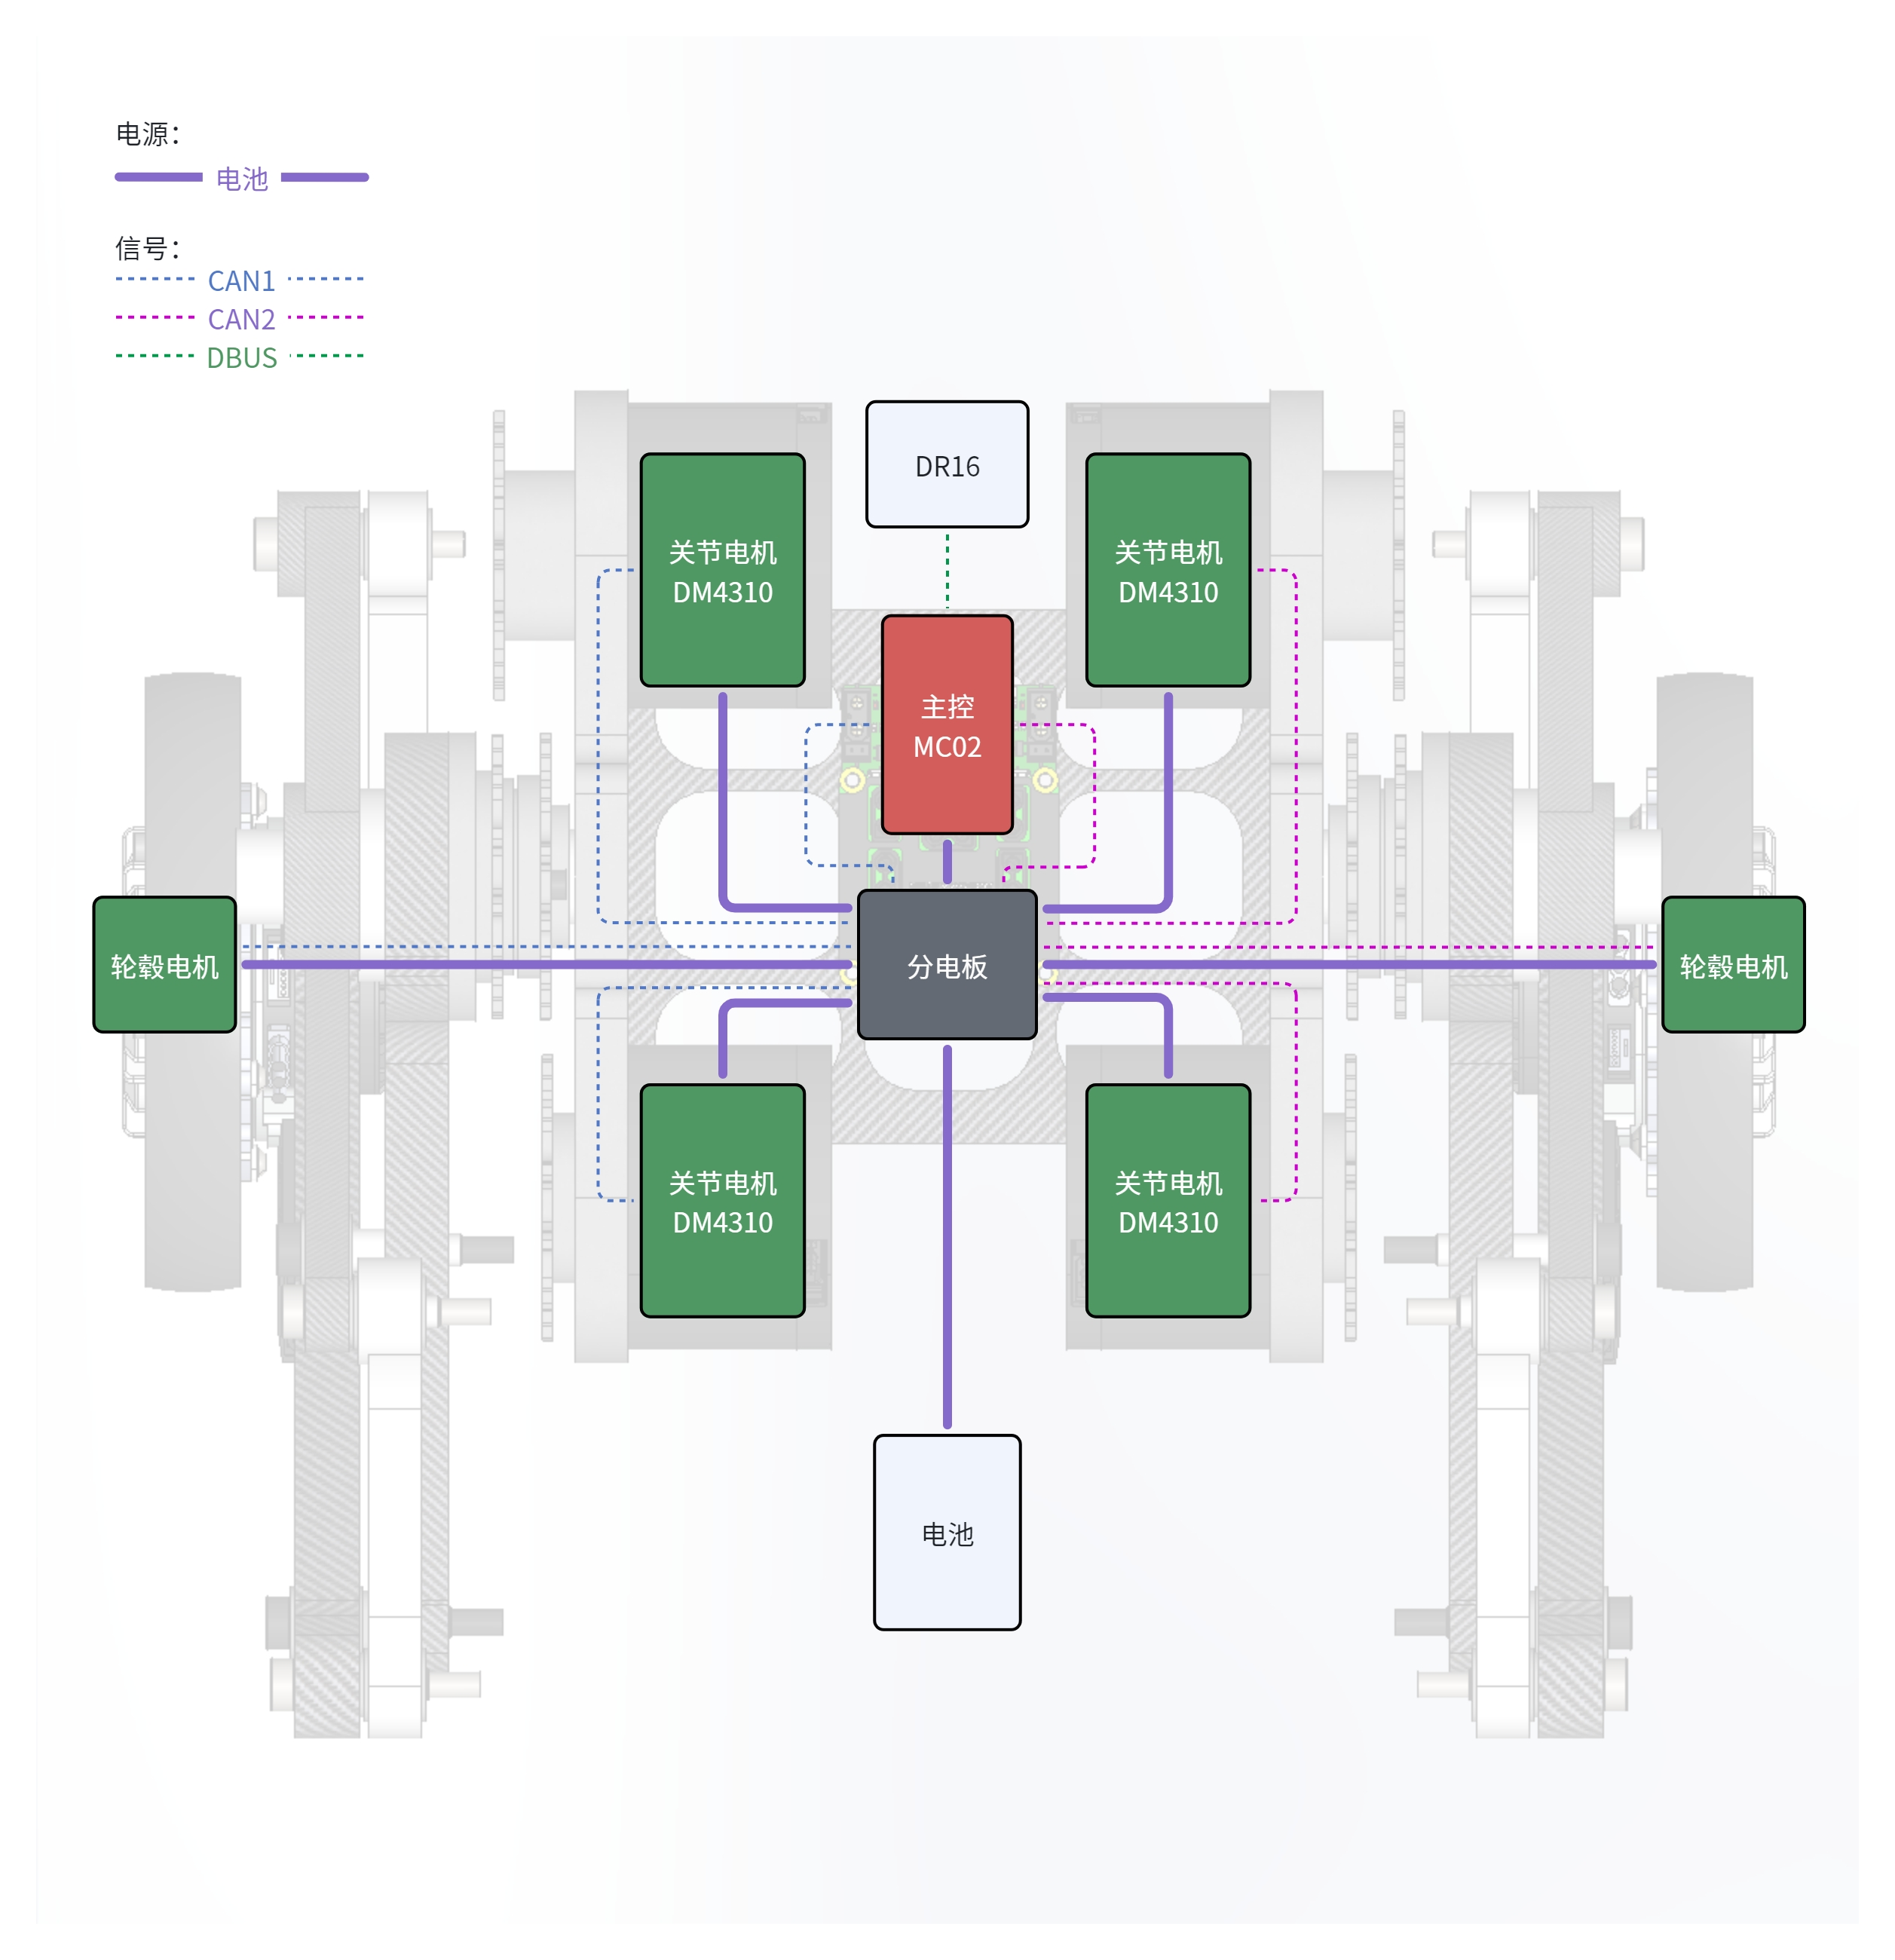
\includegraphics[width=0.7\textwidth]{figures/ch05/line.jpg}
  \caption{样机接线图}
  \label{fig:experiment-hardware}
\end{figure}

样机平台的主要参数见\tabref{tab:prototype-parameters}。这些参数与第二章的结构设计和执行器选型保持一致，是后续控制参数配置和实验结果分析的硬件基础。

\begin{table}[H]
  \centering
  \caption{物理样机主要参数}\label{tab:prototype-parameters}
  \renewcommand{\arraystretch}{1.25}
  \begin{tabular}{lcc}
    \toprule
    参数 & 数值 & 说明 \\
    \midrule
    整机质量 & 约 $3.5\,\mathrm{kg}$ & 含电池、控制板和驱动器 \\
    轮半径 & $0.06\,\mathrm{m}$ & 足端驱动轮半径 \\
    单腿主动自由度 & $2$ & 闭环连杆机构主动关节 \\
    轮端驱动自由度 & $2$ & 左右轮毂电机差速驱动 \\
    腿部关节电机峰值扭矩 & $7\,\mathrm{N\cdot m}$ & 短时输出能力 \\
    轮毂电机额定扭矩 & $2.46\,\mathrm{N\cdot m}$ & 减速箱输出端 \\
    控制频率 & $1\,\mathrm{kHz}$ & 控制器目标运行频率 \\
    \bottomrule
  \end{tabular}
\end{table}

实物实验的控制结构与仿真一致：LQR 出轮端力矩和腿摆量，VMC 出腿长支撑力，滚转环出左右腿长差修正。不同的是，实物上多了执行器带宽、轮地接触状态和传感器噪声这些仿真里吃不透的因素。所以仿真参数只能当起点，实物上还得根据实际响应再调——有的增益要收，有的限幅要放，有的方向需要反复试。

调试的基本顺序是：先离线算好 LQR 增益，把轮端限幅压到较低水平，在保护架里做小幅站立；等机器人能从不大的初始偏斜里自己回来，再逐步放开轮端力矩限幅和姿态增益。主平衡站稳后，调 VMC 的刚度 $K_l$ 和阻尼 $D_l$，原则是腿撑得住、不振荡。滚转环最后接入，腿长差修正量设一个较小的上限，避免滚转角测量噪声引起左右腿高频哆嗦。

所有实验均在平整地面上完成。每组工况重复测试多次，离线分析时剔除通信中断、保护架碰撞、轮端离地等异常片段。本文主要从以下指标观察实验结果：

\begin{enumerate}
  \item 原地平衡实验：观察机体俯仰角和腿摆角是否收敛，前进速度是否快速收敛，以及轮端力矩是否出现长期饱和；
  \item 速度跟踪实验：观察实际速度相对参考速度的响应滞后、稳态误差和超调情况，同时检查速度变化过程中机体姿态是否保持稳定；
  \item 滚转稳定实验：观察滚转角峰值、恢复过程和左右腿长参考差异，分析滚转稳定对侧向姿态的改善作用；
  \item 腿长控制实验：观察左右实际腿长对参考腿长的跟踪能力、两侧响应一致性以及高度变化对整机平衡的影响。
\end{enumerate}

\section{原地平衡性能验证}

原地平衡是双轮足机器人开展其他运动实验的基础。实验中，左右腿参考长度均设为基准腿长，期望前进速度取 $\dot{s}_d=0$，偏航角和腿摆角参考值取零。样机由初始支撑状态进入直立状态后，LQR 控制器根据俯仰角、俯仰角速度和轮系状态输出轮端力矩，使机器人通过小范围前后移动维持倒立摆平衡；VMC 控制器则维持左右腿长在基准值附近，为机体提供稳定支撑。

\begin{figure}[H]
  \centering
  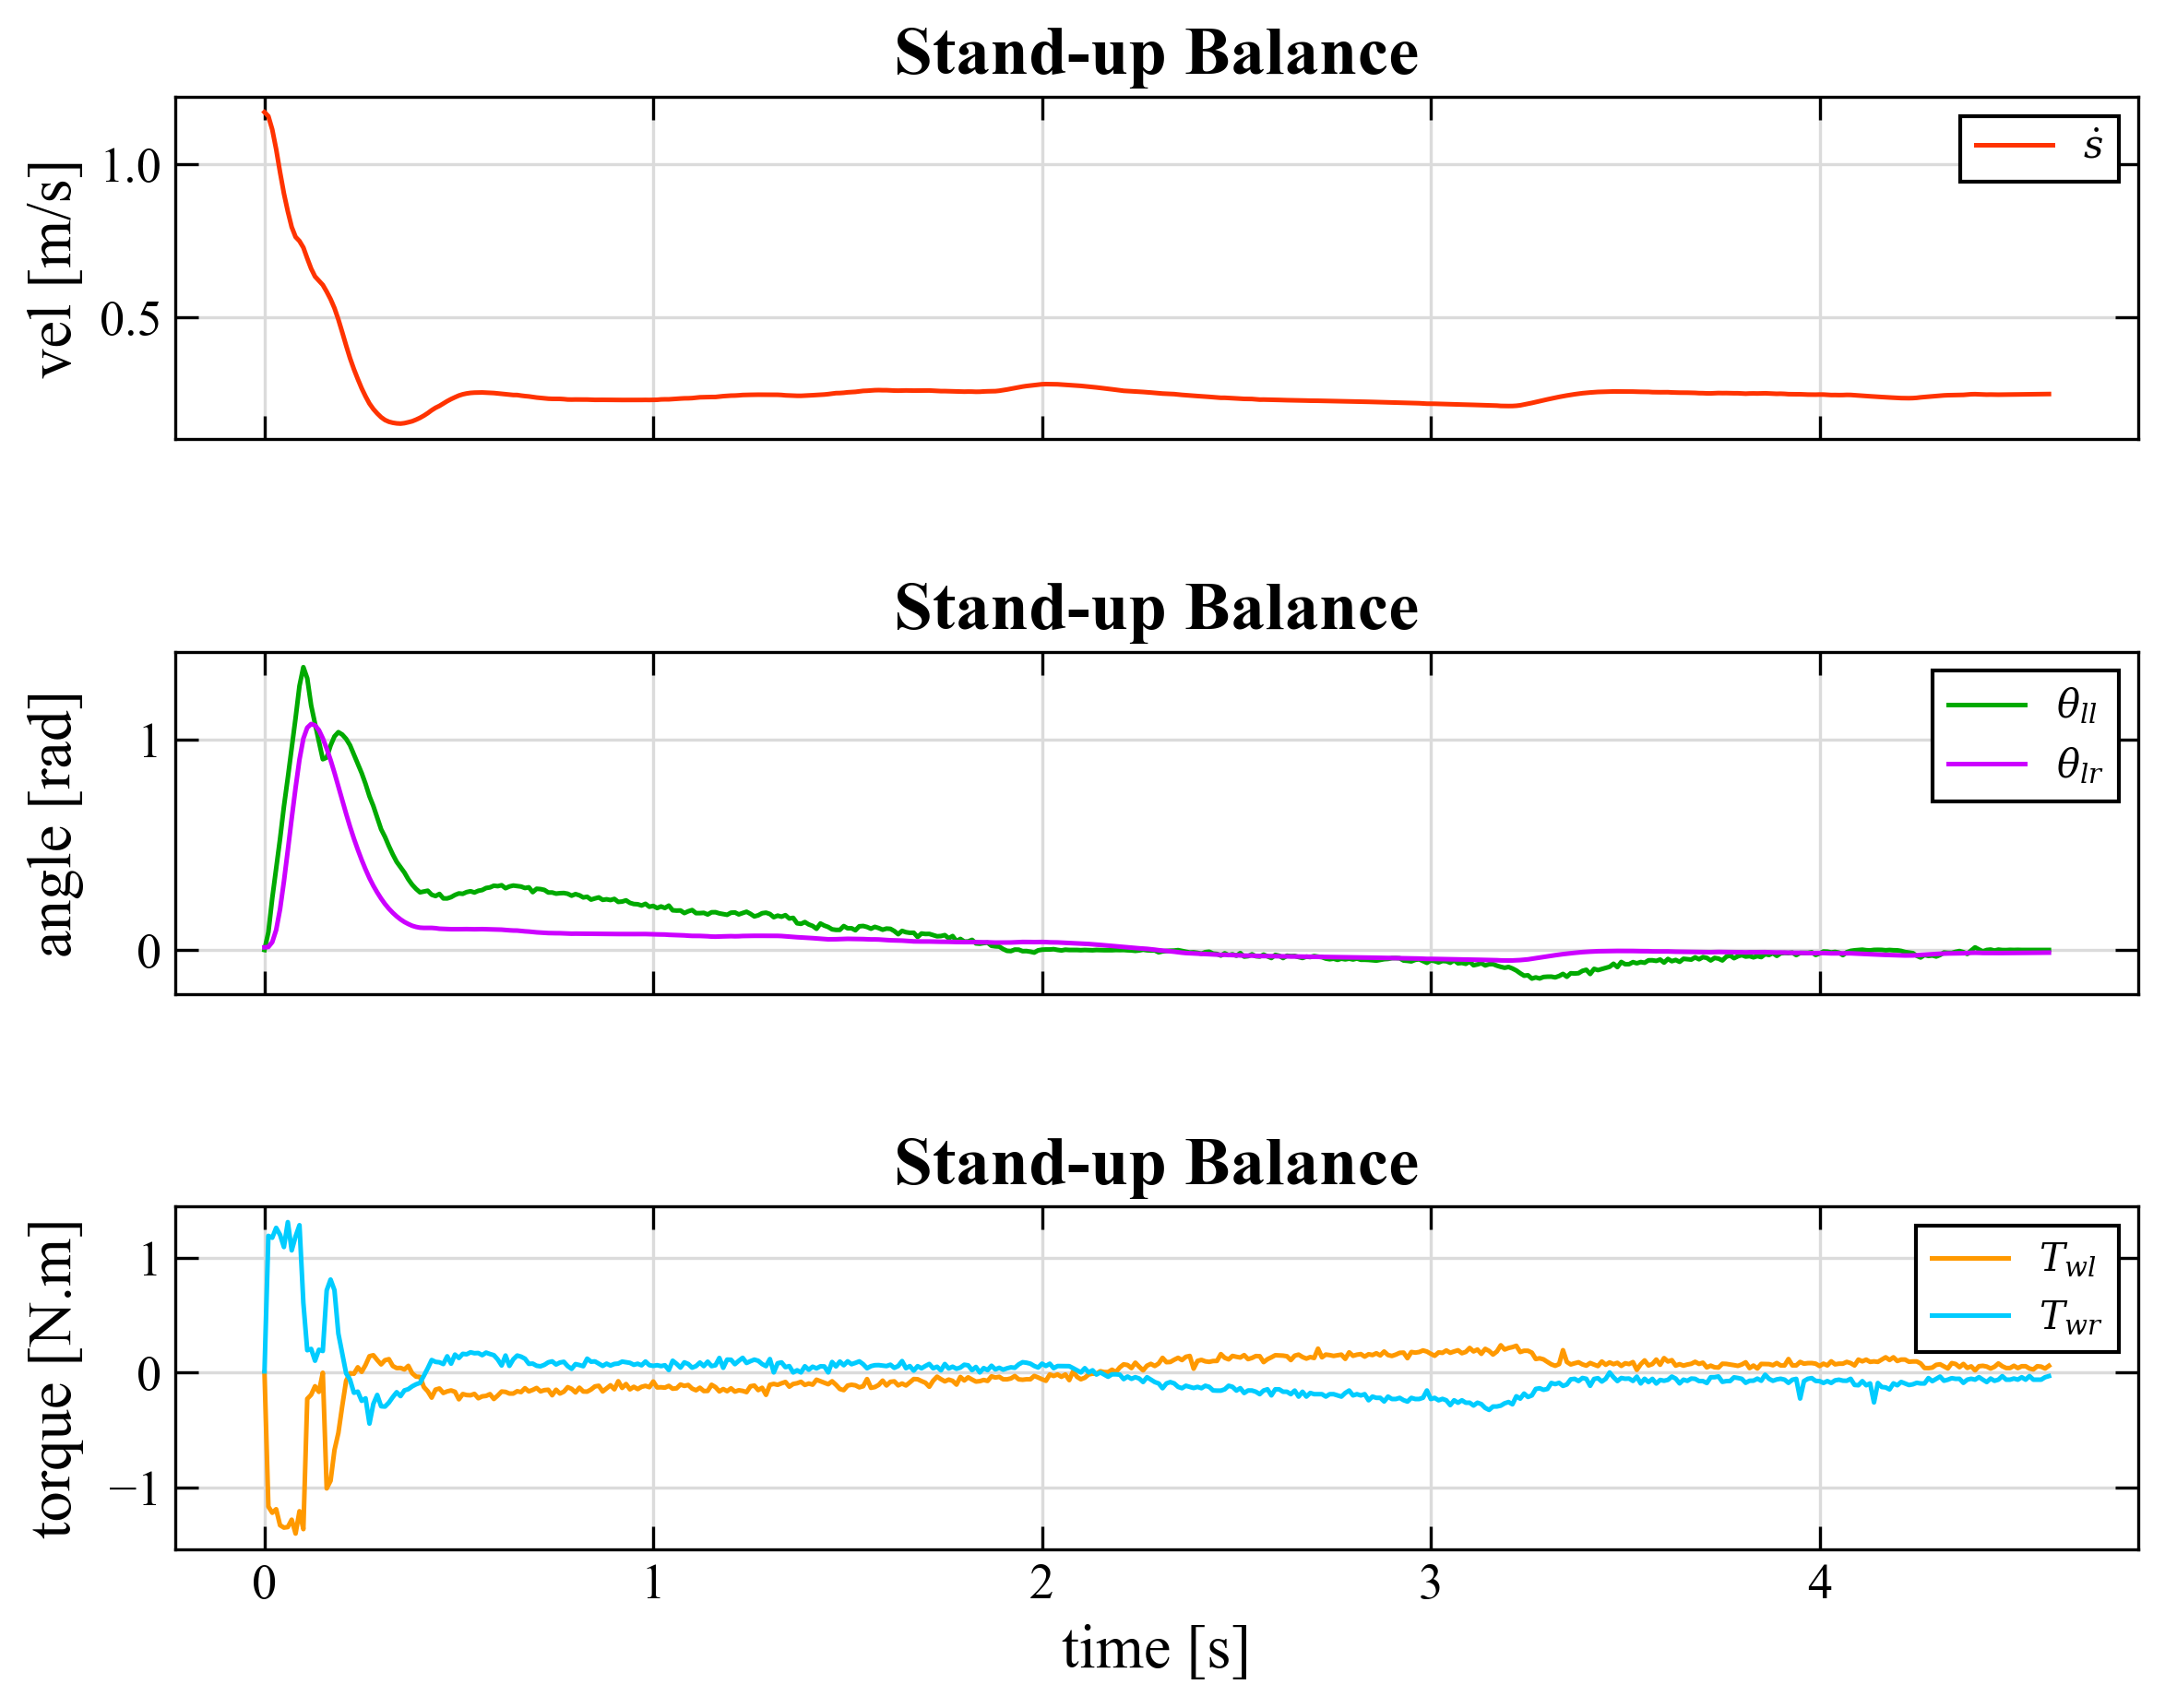
\includegraphics[width=1.0\textwidth]{figures/ch05/standup.png}
  \caption{原地平衡实验响应曲线}
  \label{fig:balance-experiment-response}
\end{figure}

\begin{figure}[H]
  \centering
  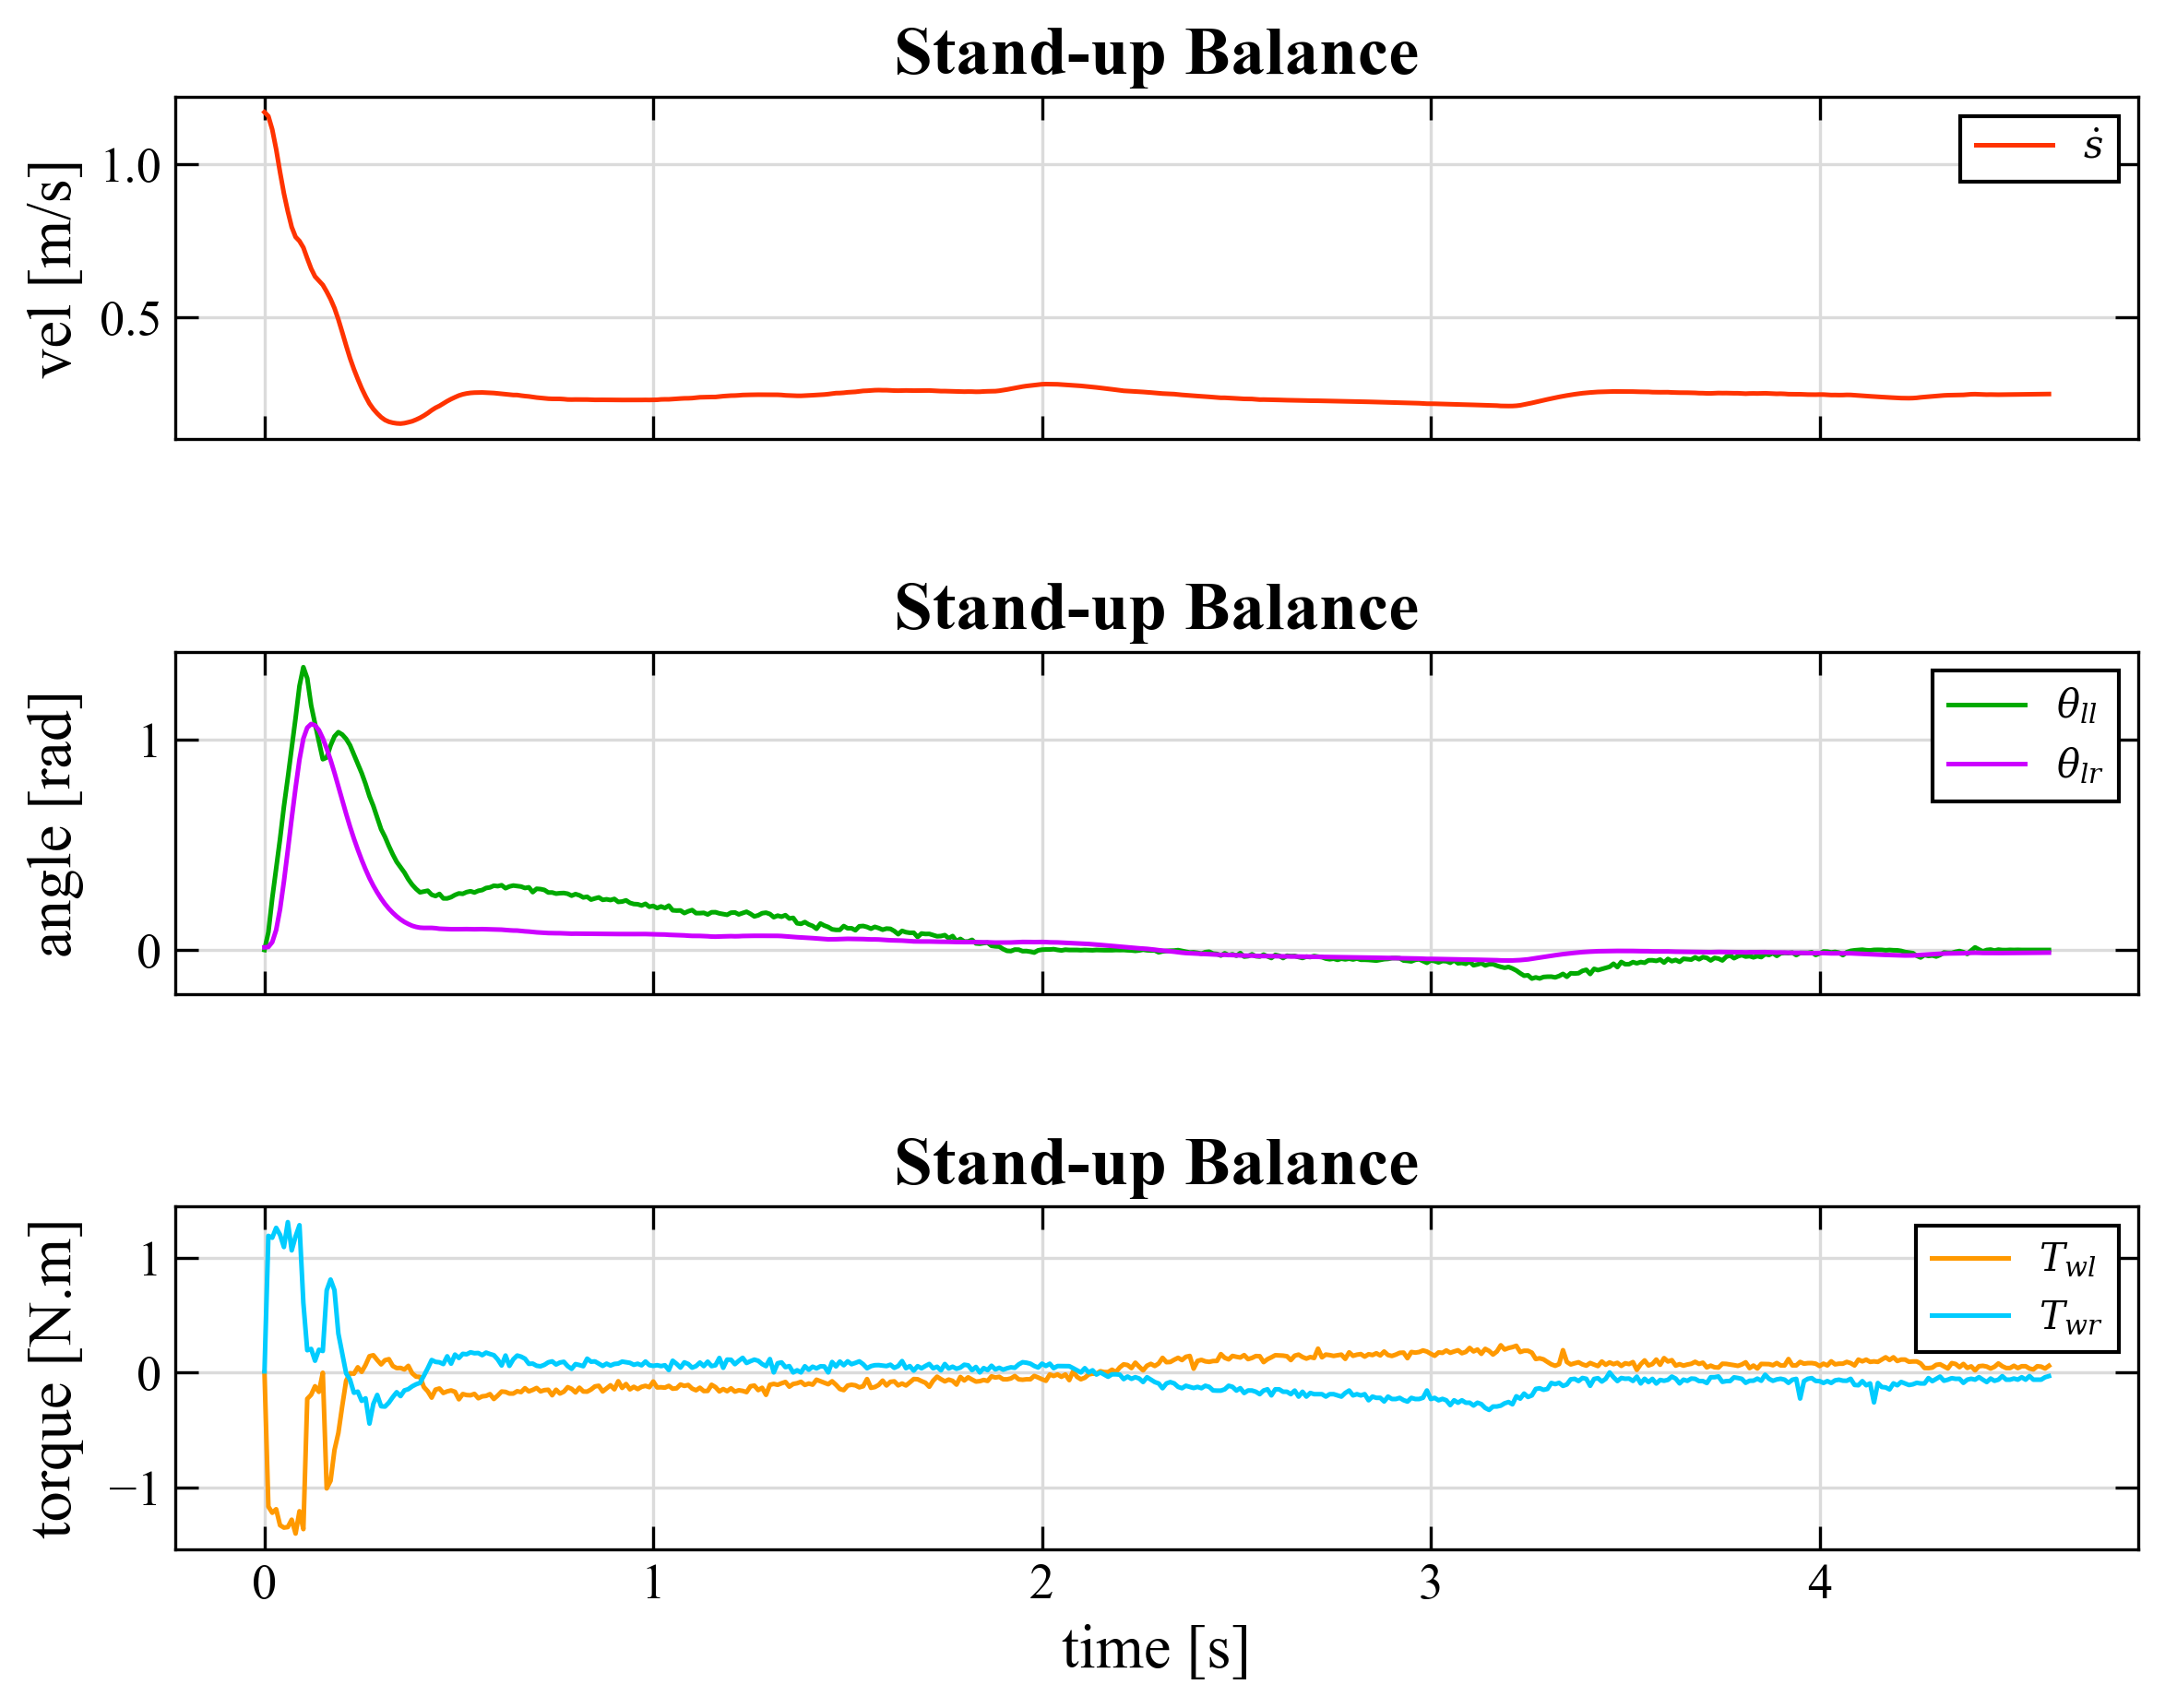
\includegraphics[width=0.6\textwidth]{figures/ch05/standup.jpg}
  \caption{原地起立并平衡过程。从上至下分别为：初始态，过渡态，平衡态}
  \label{fig:balance-experiment-scene}
\end{figure}


由\figref{fig:balance-experiment-response} 可见，起立初期机器人从支撑姿态过渡到直立姿态，前进速度和腿摆角都会出现一段较明显的瞬态变化。进入平衡阶段后，左右腿摆角回到零点附近，后续没有继续放大的低频摆动；前进速度也从起立阶段的较大变化逐渐降下来，只在零点附近小幅波动。也就是说，样机主要通过短距离前后调整来维持倒立摆平衡，并未产生明显的持续位移。

轮端力矩的变化也与这一过程一致。起立初期，两侧轮电机输出方向相反，幅值相对较大，用于快速修正机体姿态；平衡建立后，左右轮端力矩逐渐减小，并围绕零点附近波动，没有出现长时间饱和。两侧力矩曲线整体较为接近，说明样机左右传动和控制响应没有明显偏差。上述结果表明，LQR 与 VMC 在实物平台上能够配合完成原地起立和平衡保持。

\section{速度跟踪性能验证}

速度跟踪实验用于验证 LQR 控制器在速度调节和机体姿态稳定之间的协调能力。实验中，机器人先完成原地平衡，随后给定分段常值的速度参考。为降低速度指令突变对轮端摩擦和机体姿态的冲击，程序中对速度参考加入斜坡限幅。

\begin{figure}[H]
  \centering
  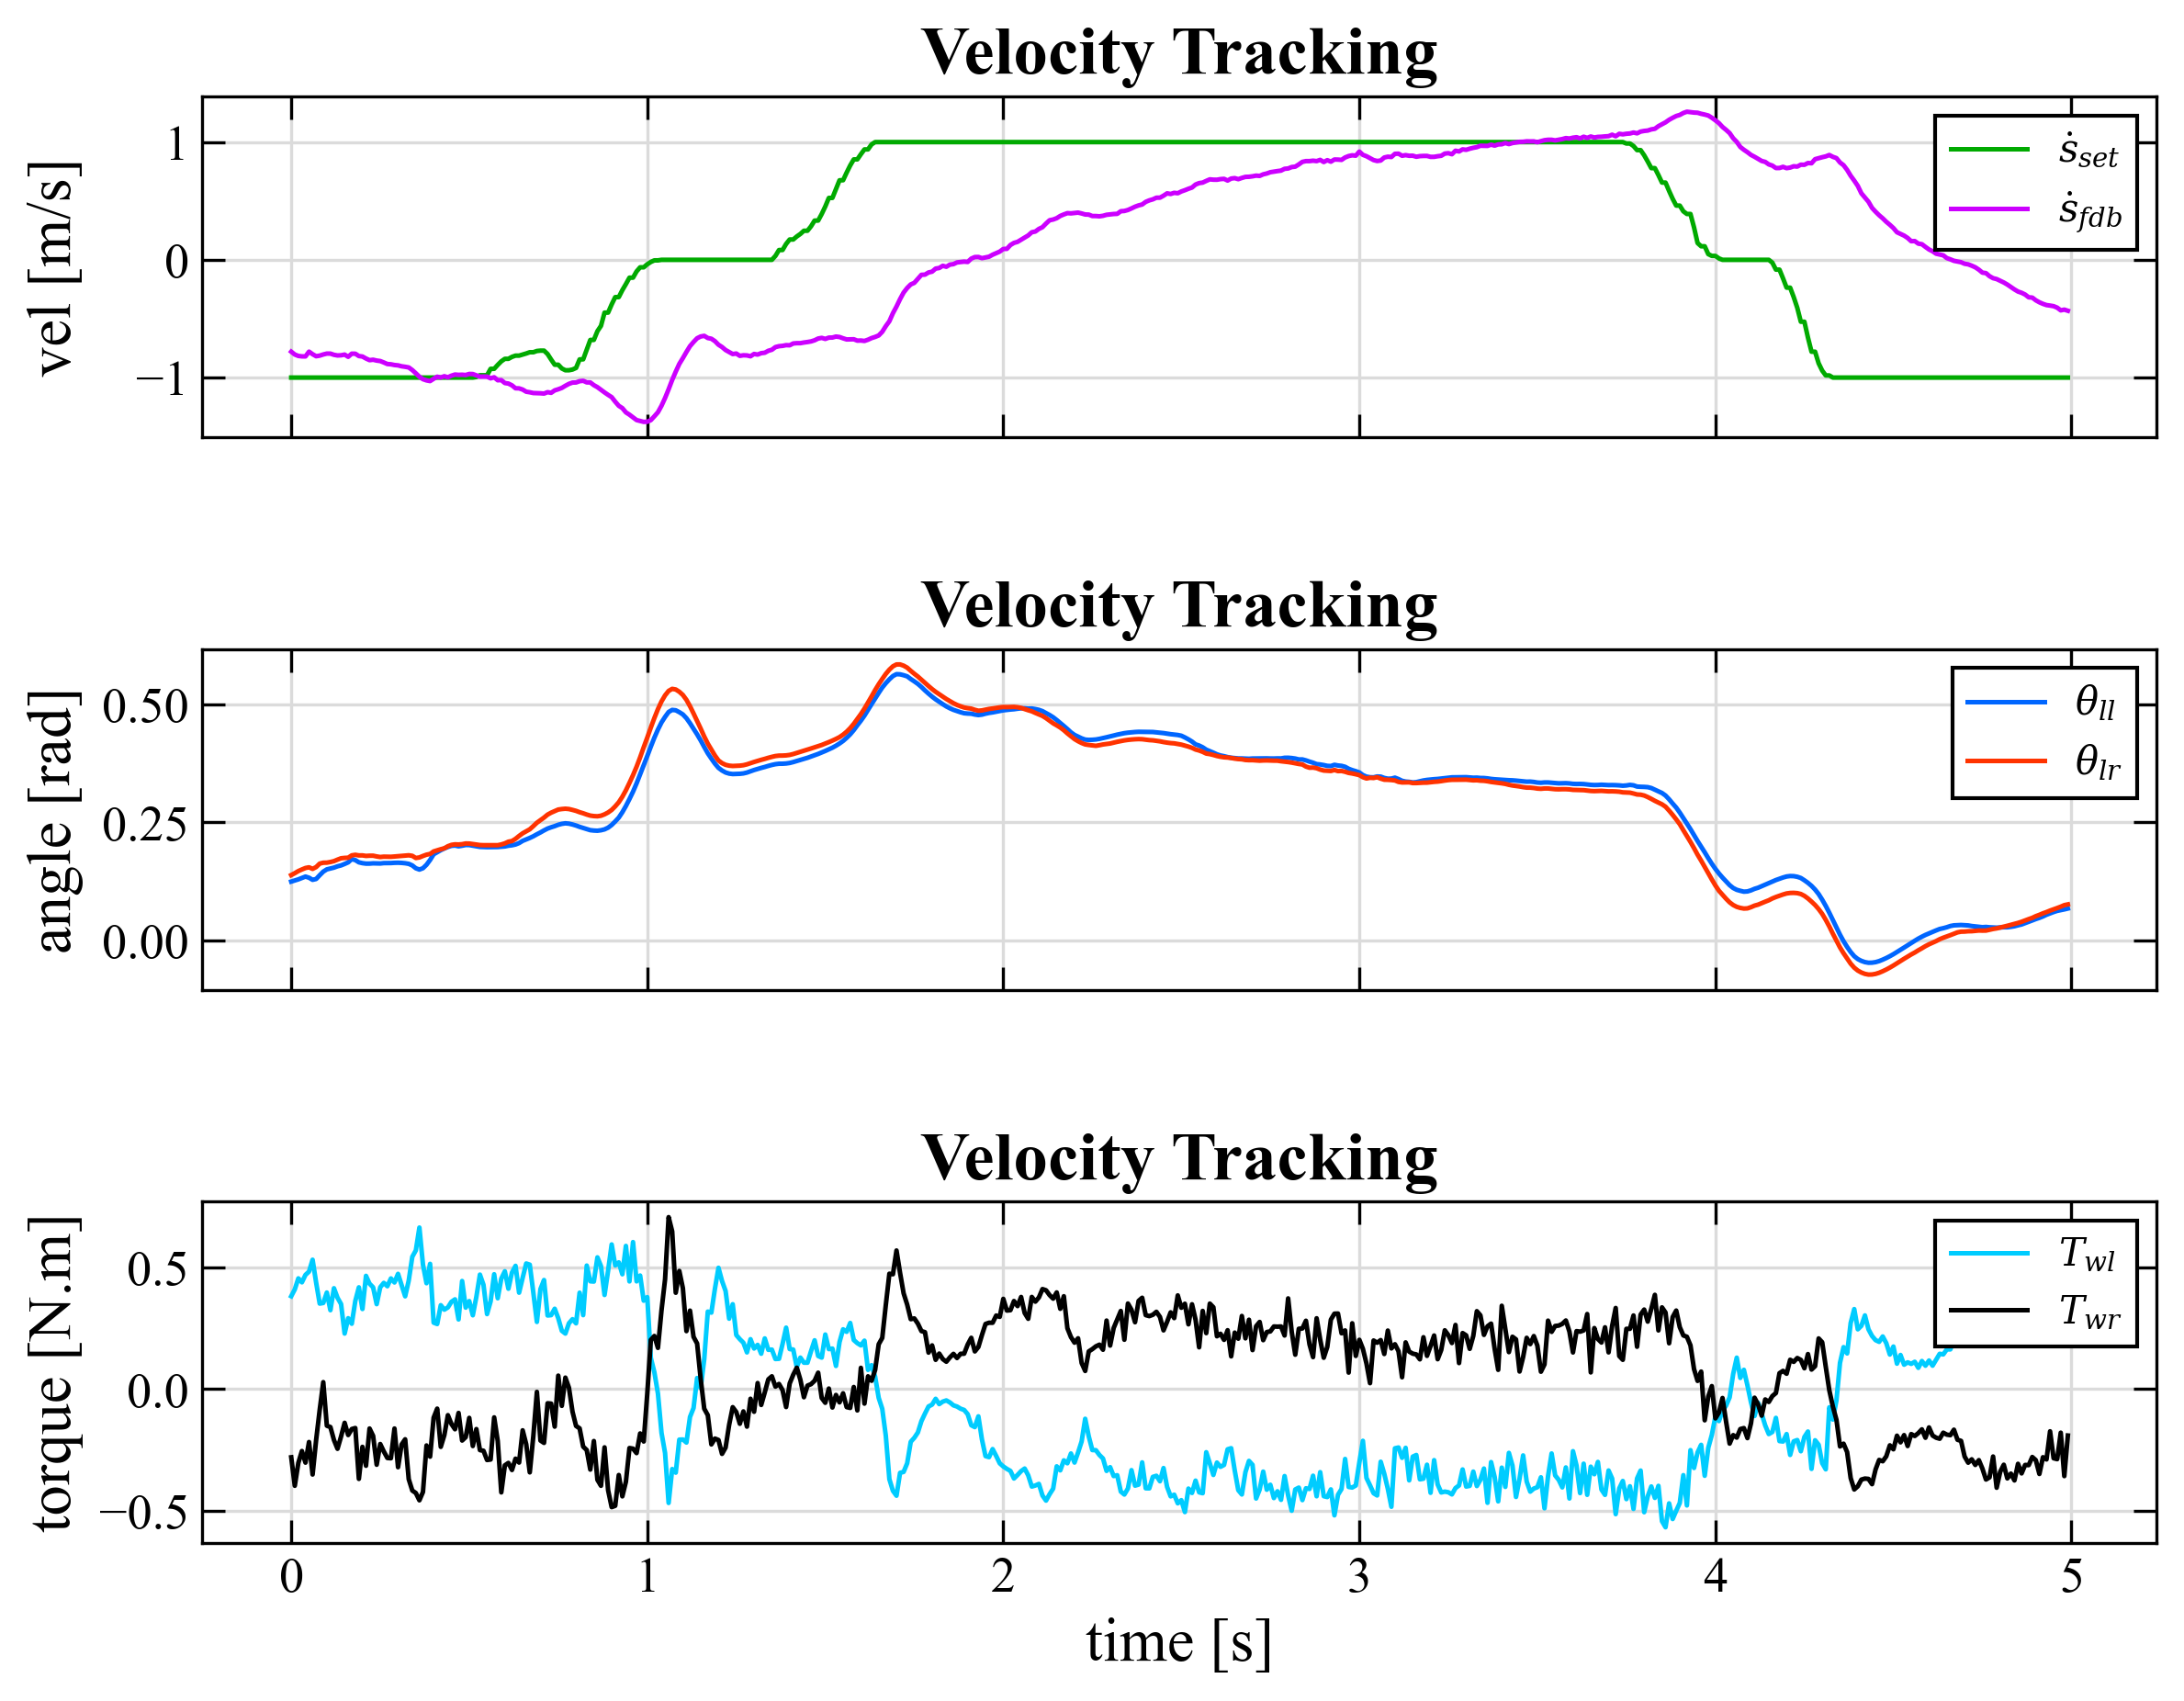
\includegraphics[width=0.9\textwidth]{figures/ch05/ds.png}
  \caption{速度跟踪实验响应曲线}
  \label{fig:velocity-experiment-response}
\end{figure}

速度跟踪实验结果如\figref{fig:velocity-experiment-response} 所示。当速度参考由负向或零附近逐渐切换至正向时，实际速度能够跟随参考速度变化，并在加速阶段呈现连续上升趋势。由于实物样机存在轮地摩擦变化、电机响应滞后和速度估计滤波延迟，实际速度相对于参考速度存在一定滞后，且在参考速度变化较快时会出现短时跟踪误差。该现象符合物理平台的实际运动特性。

\begin{figure}[H]
  \centering
  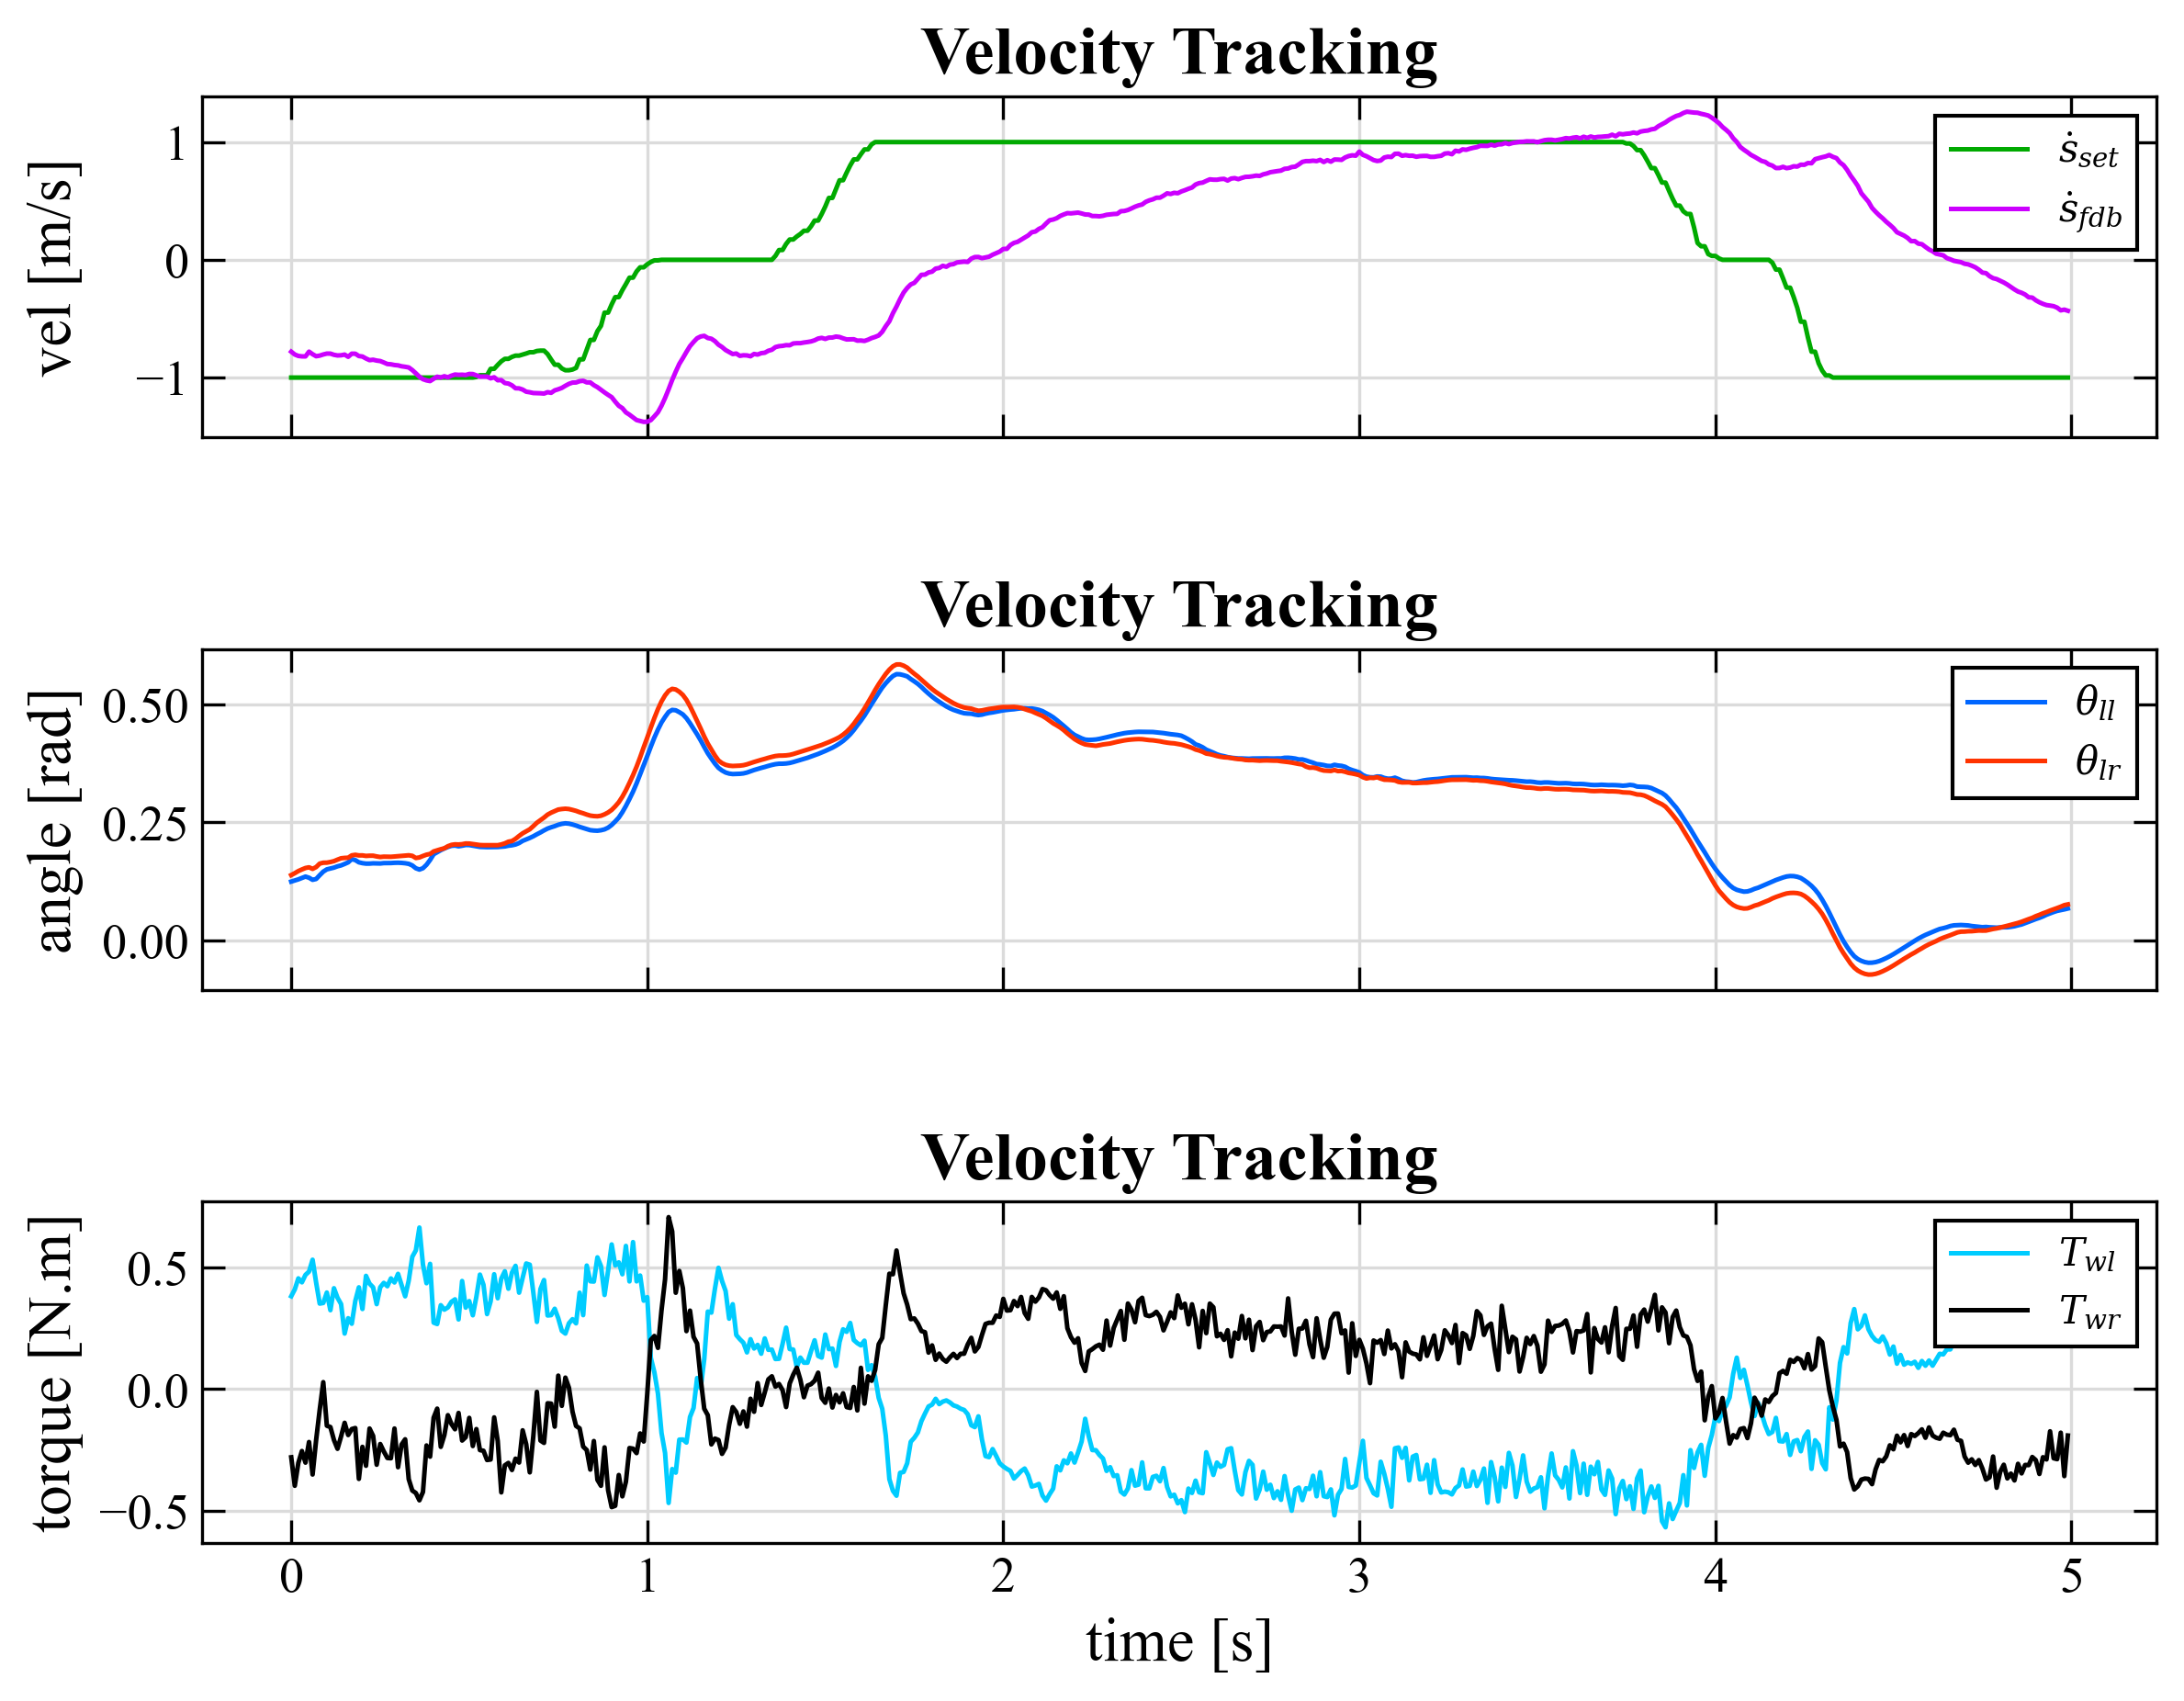
\includegraphics[width=0.5\textwidth]{figures/ch05/ds.jpg}
  \caption{速度跟踪机器人位姿表现。从上至下依次为：平衡态，加速态，匀速态}
  \label{fig:velocity-experiment-scene}
\end{figure}

速度调节期间，左右腿摆角基本同步变化，没有出现单侧腿摆明显偏离的情况。样机加减速时主要依靠机体整体前后倾斜，并配合轮端驱动力完成速度调整。当速度参考由正向切换为反向时，腿摆角会先减小，再短暂向反方向偏转，这与双轮倒立摆减速、反向时的姿态调整过程一致。轮端力矩在速度切换阶段波动较大；参考速度变化趋缓后，力矩幅值也随之回落。

\section{腿长控制验证}

腿长控制实验用于验证 VMC 腿长通道在物理样机上的高度调节和支撑能力。实验中，机器人首先保持原地平衡，随后给定左右腿公共腿长参考 $l_d$ 的周期性升降指令，并记录左右实际腿长的跟踪过程。该实验不额外改变 LQR 主控制律，腿摆方向仍由 LQR 输出控制量，因此可以较为独立地观察 VMC 腿长控制对机体高度变化的影响。

\begin{figure}[H]
  \centering
  \includegraphics[width=0.55\textwidth]{figures/ch05/leg.jpg}
  \caption{腿长控制机器人位姿表现}
  \label{fig:leg-experiment-scene}
\end{figure}

\begin{figure}[H]
  \centering
  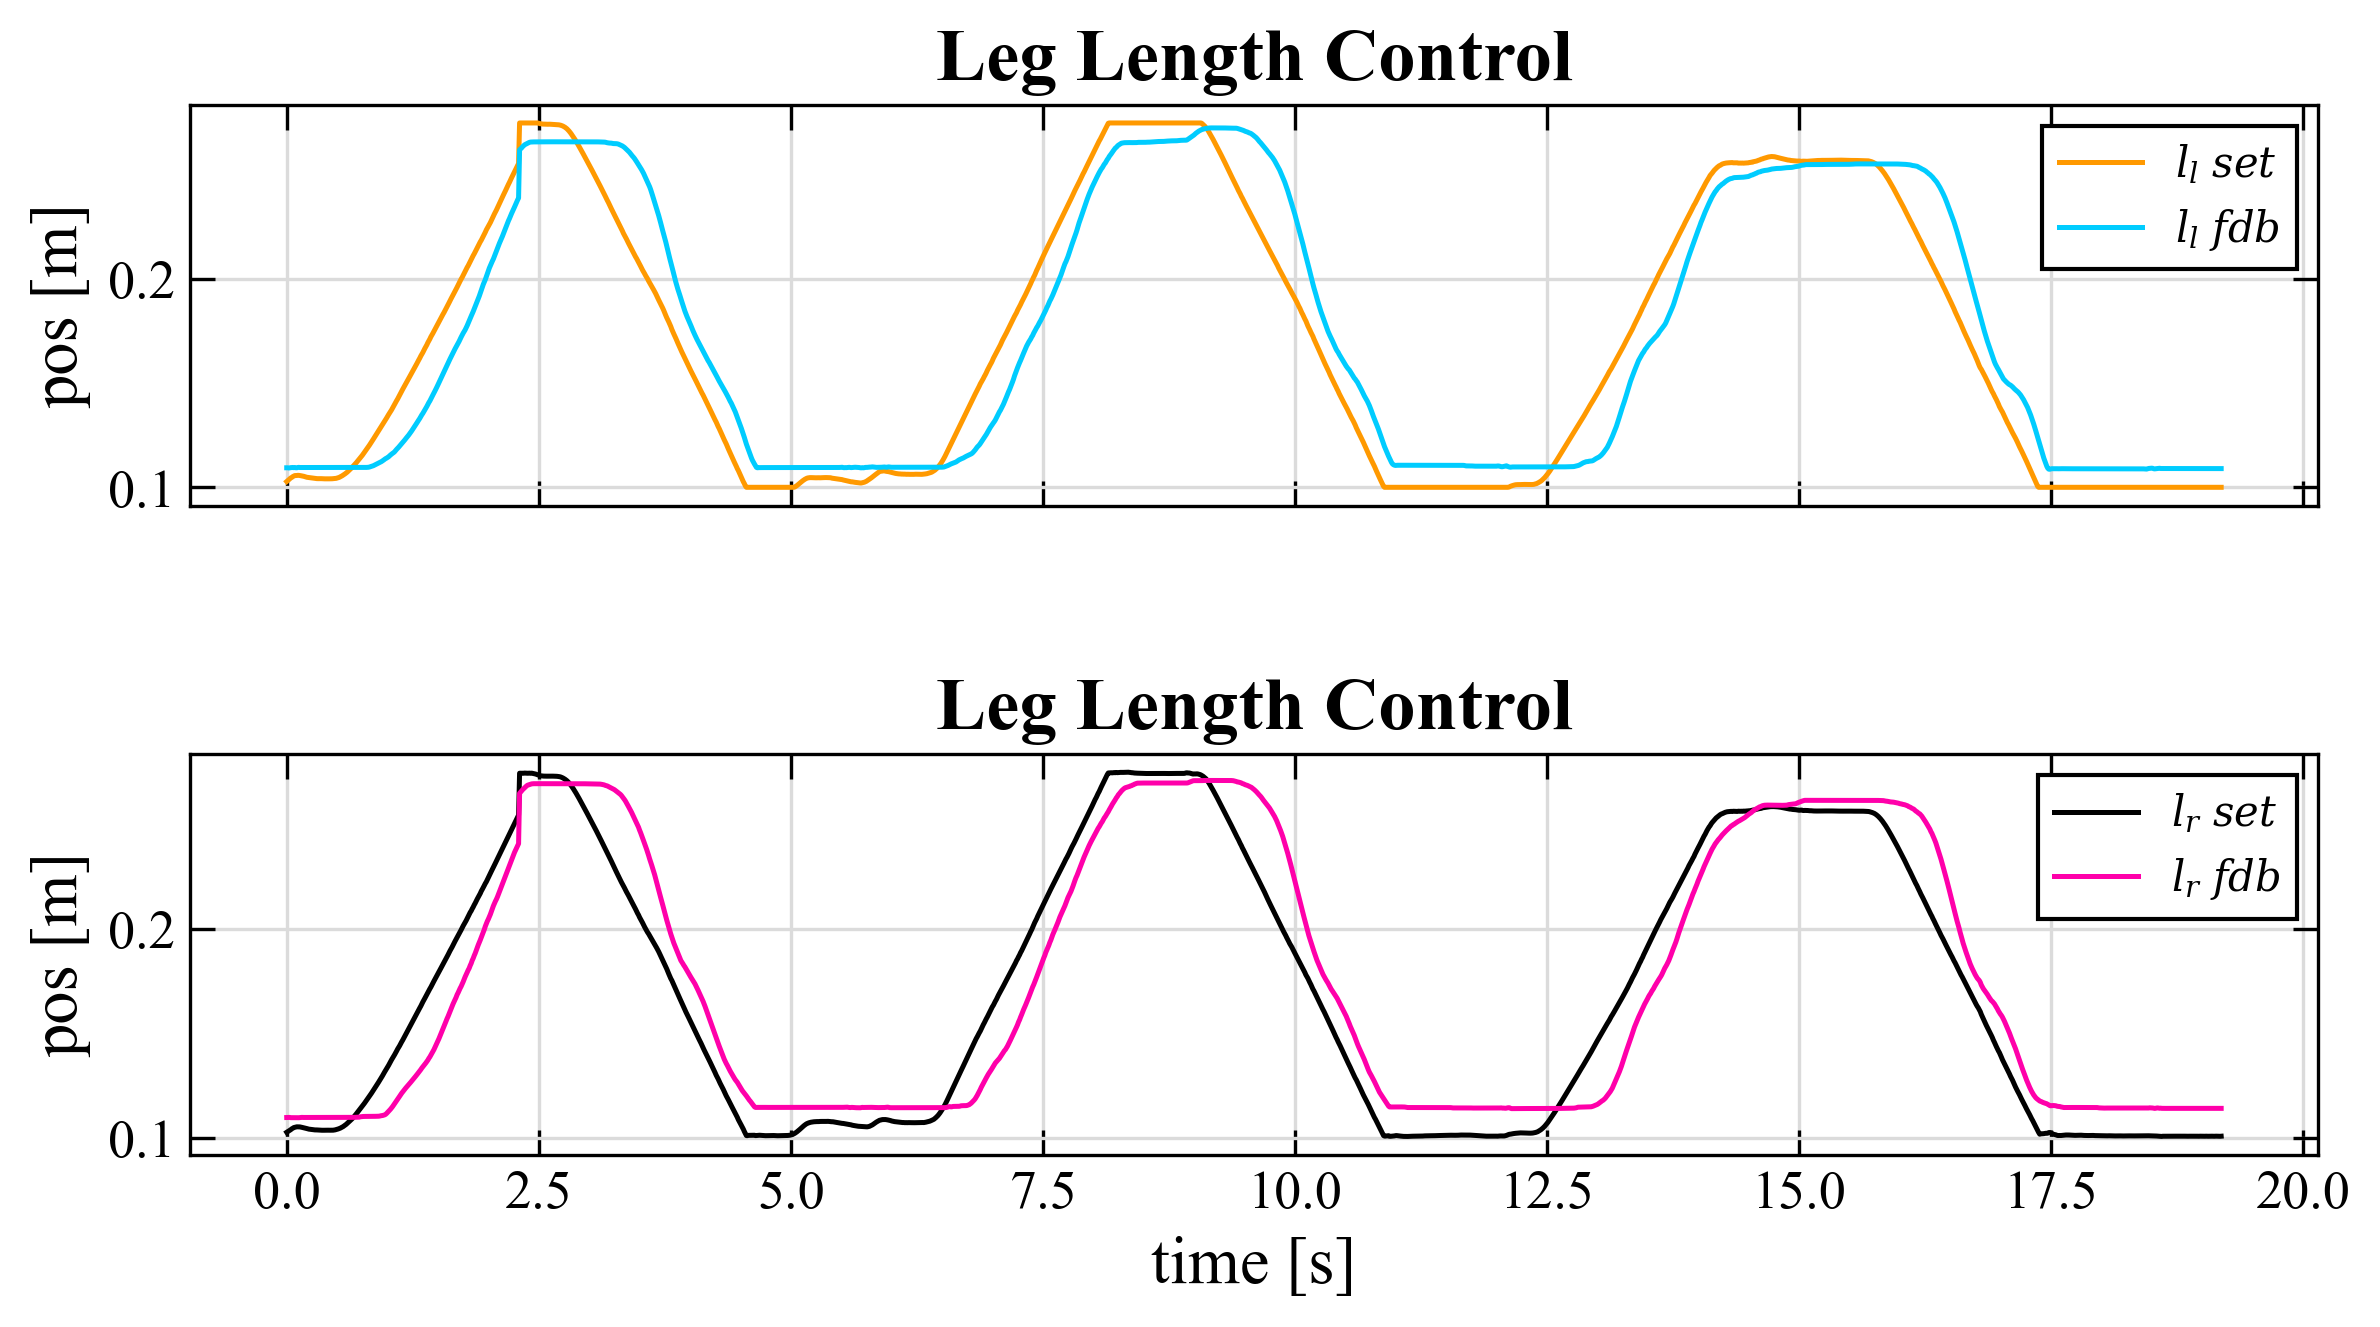
\includegraphics[width=0.8\textwidth]{figures/ch05/leg_control.png}
  \caption{腿长控制实验响应对比}
  \label{fig:leg-experiment-response}
\end{figure}

由\figref{fig:leg-experiment-response} 可见，左右腿参考长度在低位和高位之间周期性切换，实际腿长也随之完成伸长和缩短。两侧响应趋势接近，没有出现一侧明显快于另一侧或长期偏离参考值的情况，说明腿部机构装配和驱动参数整体比较一致。该结果也表明，第三章的腿部运动学解算和第四章的 VMC 腿长控制律可以在样机上闭环运行。

实际腿长相对于参考腿长仍存在一定滞后，尤其在参考值快速上升或下降时更明显。这一部分滞后主要来自电机响应、链传动间隙、腿部连杆惯量以及程序中的指令限幅。进入高位或低位保持阶段后，实际腿长能够停留在参考值附近，没有持续振荡。由此可见，当前虚拟弹簧阻尼参数没有单纯追求最快响应，而是在响应速度和稳定性之间取了较保守的设置。继续增大腿长刚度可以缩短调节时间，但会提高关节力矩峰值，也更容易激发结构振动；阻尼过大则会让腿长变化变慢。因此，实物调参时需要同时看腿长误差、关节力矩和机体姿态变化。

在腿长周期性升降的过程中，机器人仍能保持基本平衡，未出现由高度调节引起的明显俯仰失稳。这说明 VMC 腿长通道接入后没有破坏 LQR 主平衡闭环。也就是说，腿长支撑和倒立摆平衡可以通过任务空间力矩映射同时作用在腿部执行器上，实验结果与第四章的分层控制设计相符。

\section{滚转稳定性能验证}

第三章建立的主动力学模型主要描述机器人前进方向、腿摆和机体俯仰之间的耦合关系，并未将滚转角直接纳入 LQR 主控制器。实际样机在侧向扰动、转向或左右支撑高度不一致的情况下，机体会产生滚转角偏差，进而导致左右腿支撑状态不同。本节通过滚转稳定实验验证第四章提出的基于腿长差修正的侧向稳定方法。

实验中，样机在保持主平衡控制闭环的同时开启滚转稳定。滚转稳定根据测得的机体滚转角和当前腿部几何关系，计算左右腿期望腿长差，并将其叠加到左右腿长参考值中。与直接构造侧向力矩的方法相比，该补偿方式不改变 LQR-VMC 主控制框架，仅通过调整左右支撑几何关系抑制机体侧倾，因而具有实现简单、计算量小的特点。

\begin{figure}[H]
  \centering
  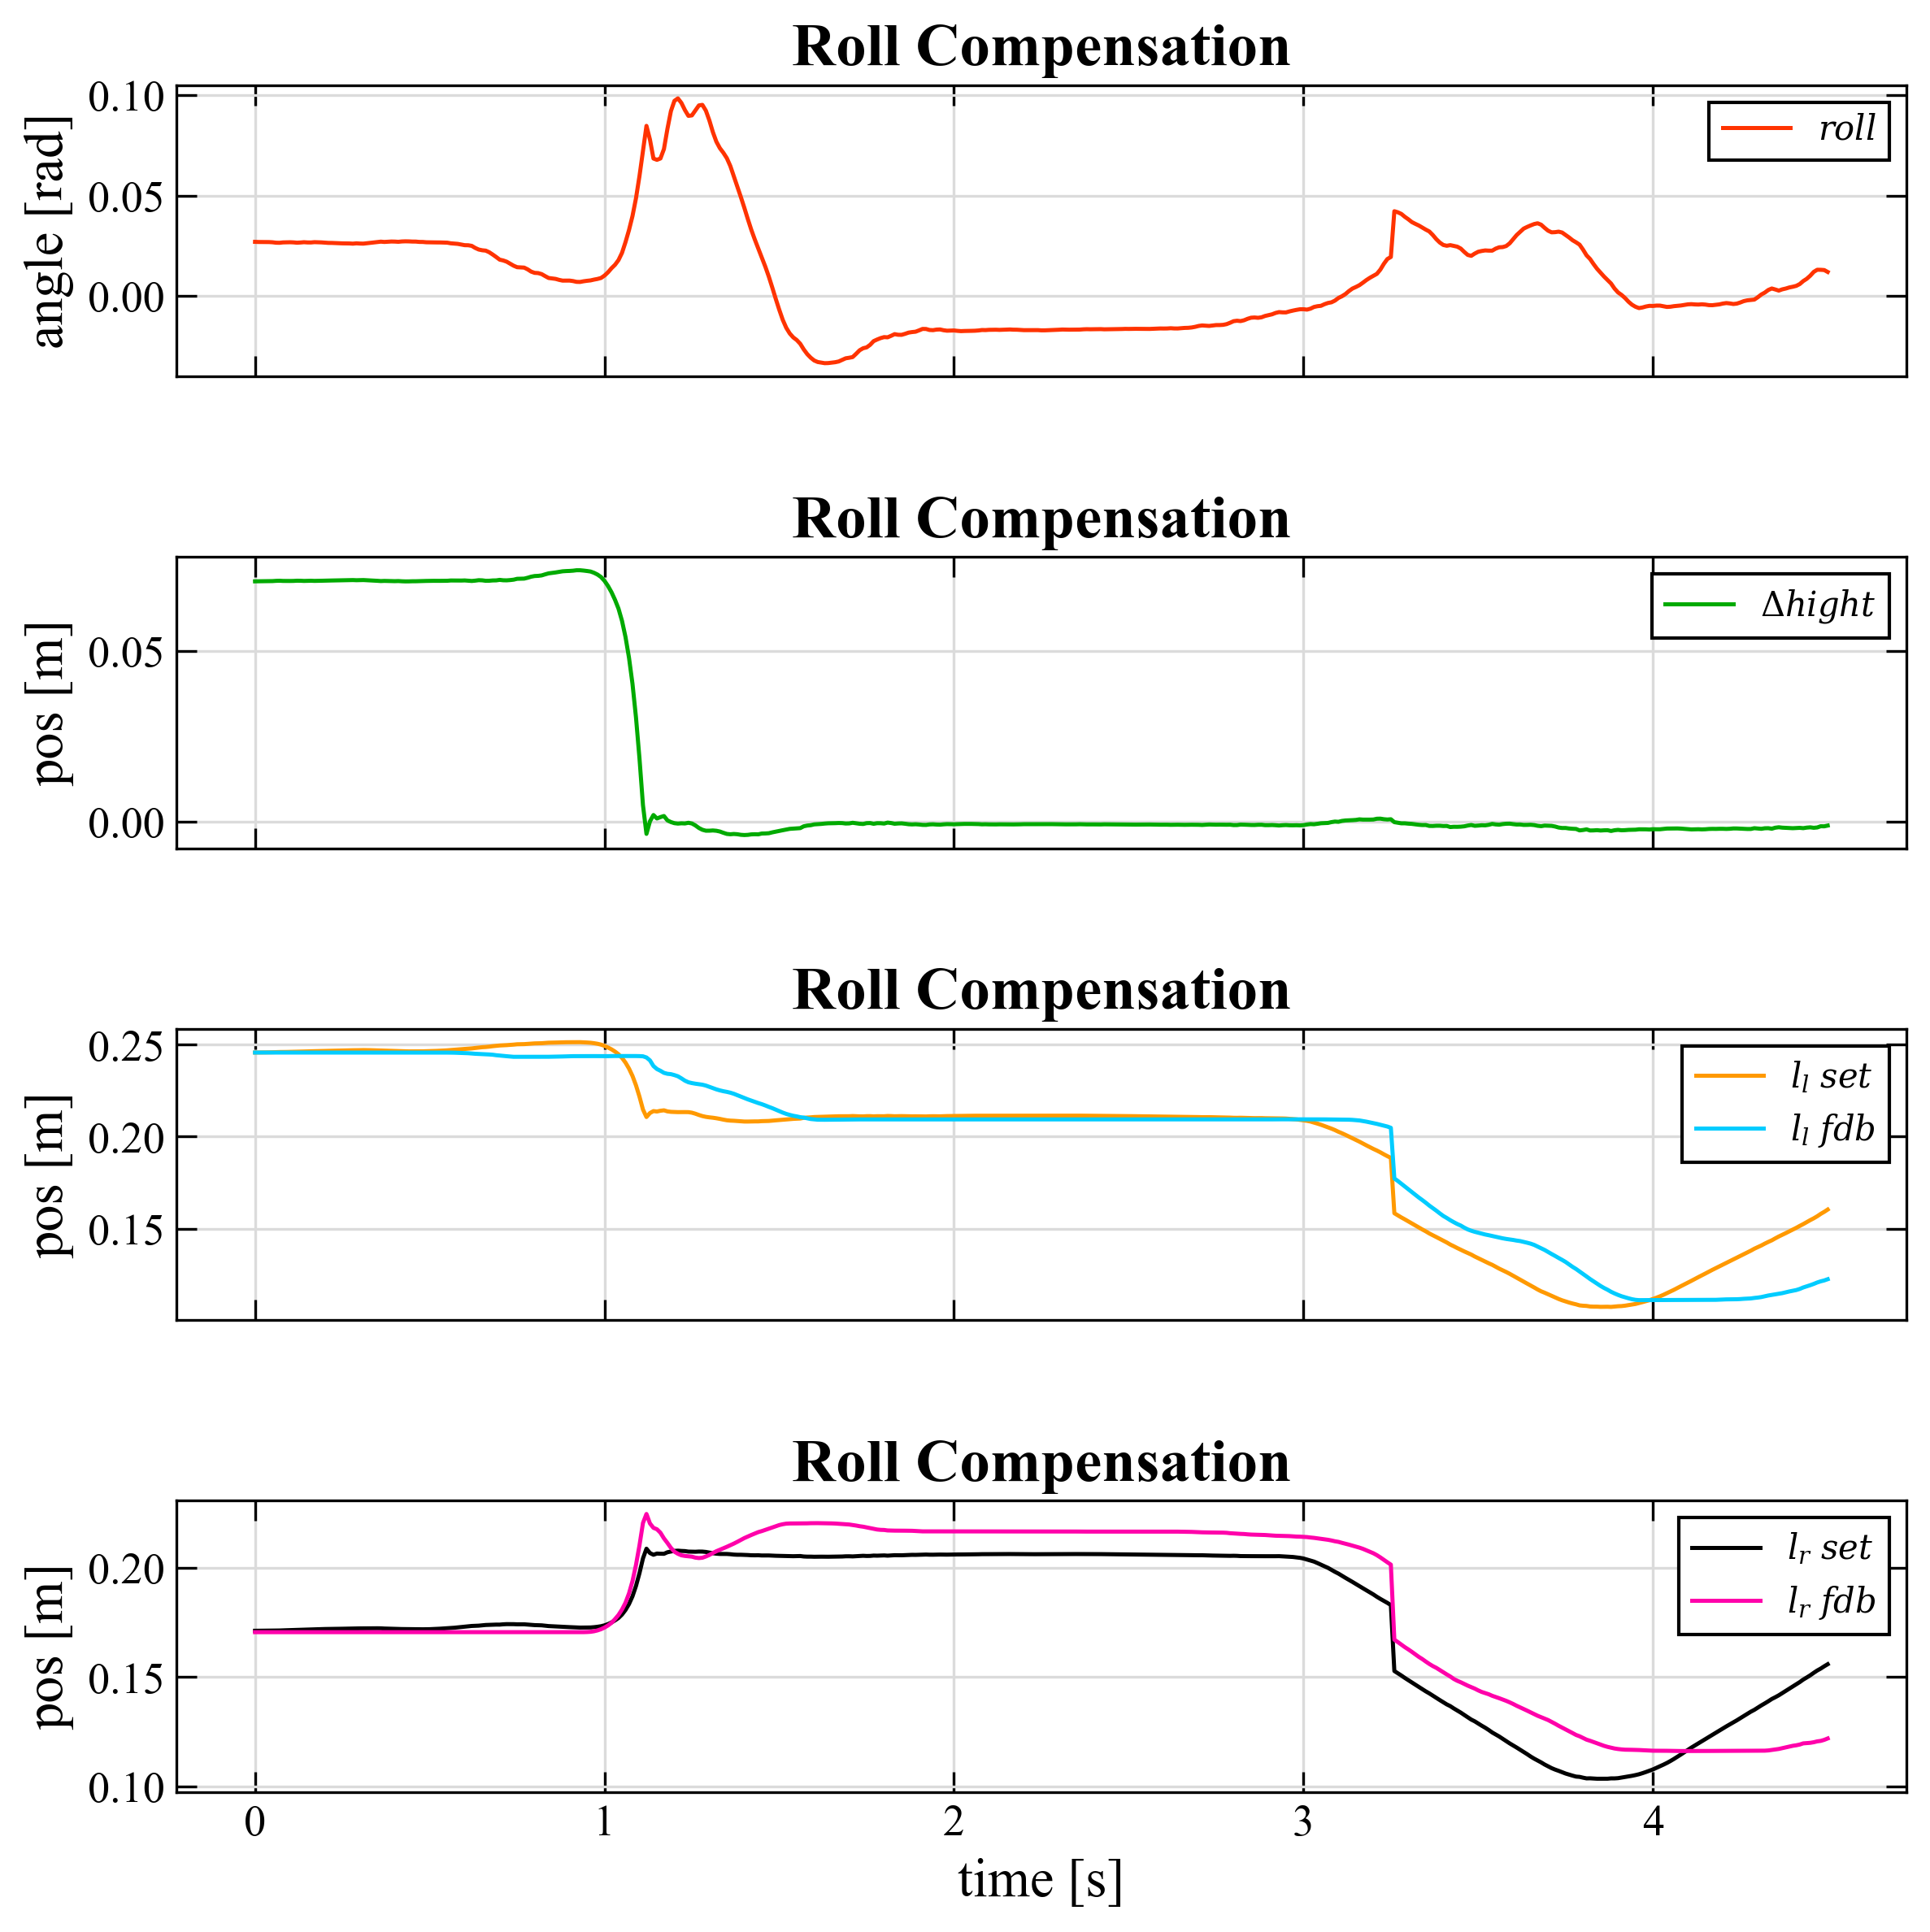
\includegraphics[width=0.7\textwidth]{figures/ch05/roll_compensation.png}
  \caption{滚转稳定前后实验响应对比}
  \label{fig:roll-experiment-response}
\end{figure}

滚转稳定实验结果如\figref{fig:roll-experiment-response} 所示。实验过程中，机体滚转角在扰动作用下出现明显偏移，随后逐渐回到零点附近。与此同时，左右腿长参考值不再保持完全相同，而是根据滚转角变化形成相反方向的修正量。该现象说明滚转稳定环节已经参与腿长通道控制，并能够通过改变左右腿支撑高度对机体侧倾进行修正。

实验结果表明，基于腿长差修正的滚转稳定能够在不改变主控制框架的前提下改善样机侧向姿态。该方法适合用于平地低速运动和轻微侧向扰动场景，但对于高速转向、强侧向冲击或复杂三维地形，仍需结合更完整的侧向动力学模型和接触力分配策略进一步优化。

\begin{figure}[H]
  \centering
  \includegraphics[width=0.6\textwidth]{figures/ch05/roll.jpg}
  \caption{滚转稳定机器人位姿表现}
  \label{fig:roll-experiment-scene}
\end{figure}

\section{本章小结}

本章在物理样机上验证了第四章设计的 LQR-VMC 分层控制器。表\ref{tab:experiment-summary} 汇总了各工况下的关键定量指标。

\begin{table}[H]
  \centering
  \caption{各工况关键实验指标汇总}
  \label{tab:experiment-summary}
  \small
  \begin{tabular}{p{2.4cm}p{2.6cm}p{2.6cm}p{2.6cm}p{2.6cm}}
    \toprule
    指标 & 原地平衡 & 速度跟踪 & 腿长控制 & 滚转稳定 \\
    \midrule
    核心验证目标 & LQR+VMC 联合起立与平衡 & 速度 + 姿态协调 & VMC 腿长通道闭环 & 滚转角补偿有效性 \\
    \hline
    姿态稳态误差 & 俯仰角波动在 $\pm 2^\circ$ 以内（RMS 约 $1.0^\circ$--$1.5^\circ$） & 加减速期间俯仰角变化 $3^\circ$--$5^\circ$，匀速段回落至 $\pm 2^\circ$ & 高度调节期间俯仰未失稳，腿长变化对平衡的耦合在可控范围内 & 滚转角 RMS 从补偿前的约 $2.5^\circ$ 降至补偿后的约 $1.5^\circ$ \\
    \hline
    跟踪/响应性能 & 起立至平衡建立约 1--2\,s & 速度跟踪延迟约 150--300\,ms，稳态误差低于 0.05\,m/s & 腿长跟踪延迟 200--400\,ms，稳态误差在 ±3\,mm 以内 & — \\
    \hline
    执行器状态 & 平衡后轮力矩未饱和，峰值约 60\%--70\% 额定值 & 加减速阶段力矩波动较大，匀速段回落 & 关节力矩峰值由腿长刚度和速度共同决定 & 腿长差修正量在 ±5\,mm 以内 \\
    \hline
    主要局限 & 链传动间隙引入微小抖动 & 轮地摩擦变化影响稳态精度 & 快速伸缩时滞后较大 & 对快速侧向扰动响应有限 \\
    \bottomrule
  \end{tabular}
\end{table}

原地平衡实验中，样机能够完成起立并保持站立，俯仰角 RMS 值约 $1.0^\circ$--$1.5^\circ$，轮端力矩未出现长期饱和。速度跟踪实验中，实际速度可以跟随参考变化，跟踪延迟在 150--300\,ms 量级，机体姿态保持稳定。腿长控制实验中，VMC 腿长通道实现了高度调节和支撑功能，稳态腿长误差在 ±3\,mm 以内。滚转稳定实验中，滚转角补偿使 RMS 滚转角从约 $2.5^\circ$ 降至约 $1.5^\circ$，验证了基于几何关系的腿长差修正对侧向稳定性的实际改善效果。

实物实验也暴露出仿真中不明显的问题：链传动间隙带来约 50--100\,ms 的腿长响应滞后，轮地接触状态变化造成速度估计的短时波动（尤其在加减速转换阶段），滚转补偿对快速侧向扰动的响应受限于传感器带宽和腿部执行器的速度上限。上述问题与样机的机械精度、传感器配置和执行器性能直接相关，后续需从结构刚度、执行器带宽、状态估计和三维稳定控制等方面继续改进。
